\question{Câu 2}

 Cho mạch khuếch đại tín hiệu như hình vẽ. Các tụ $C_{1}$, $C_{2}$ có giá trị rất lớn. BJT có hệ số $\beta = 80$ và có mã là 2N2907.
 
 \begin{figure}[H]
 	\centering
	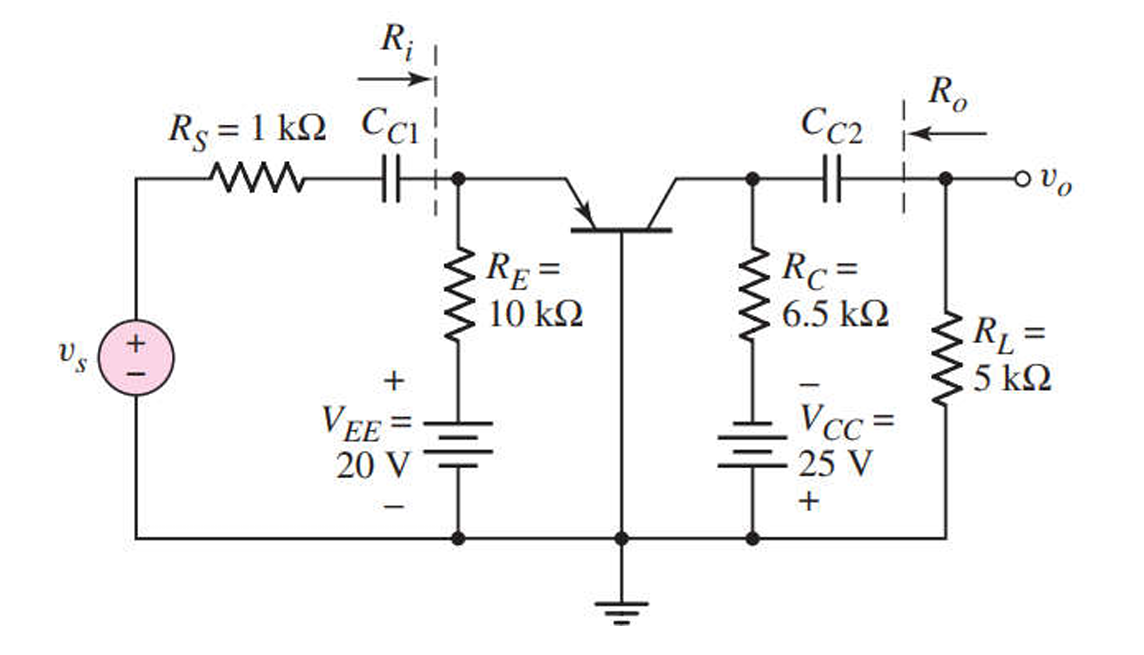
\includegraphics[width=.8\linewidth]{./my-chapters/my-images/Question2/debai.png}
 \end{figure}
 
\answer{a}{Vẽ VTC của mạch (kiểm chứng sử dụng mô phỏng) và tìm điểm hoạt động $Q$ của BJT.}

Vẽ VTC của mạch

\begin{figure}[H]
	\centering
	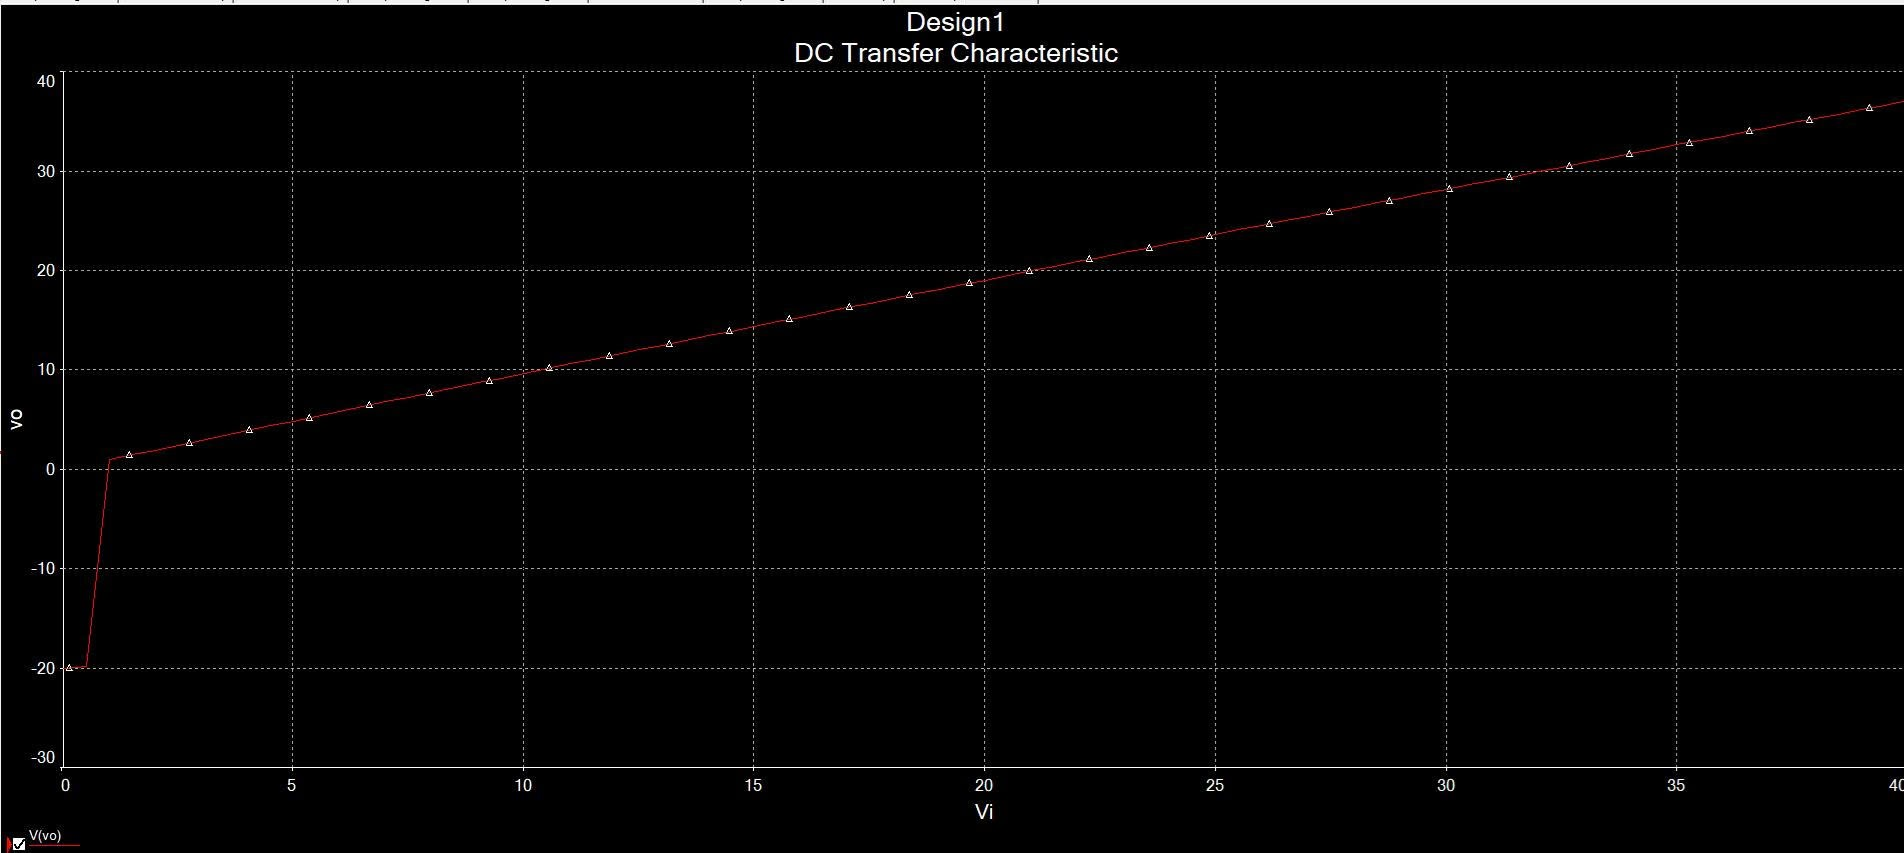
\includegraphics[width=.9\linewidth]{./my-chapters/my-images/Question2/a_VTC.png}
\end{figure}

\begin{minipage}{.4\linewidth}
	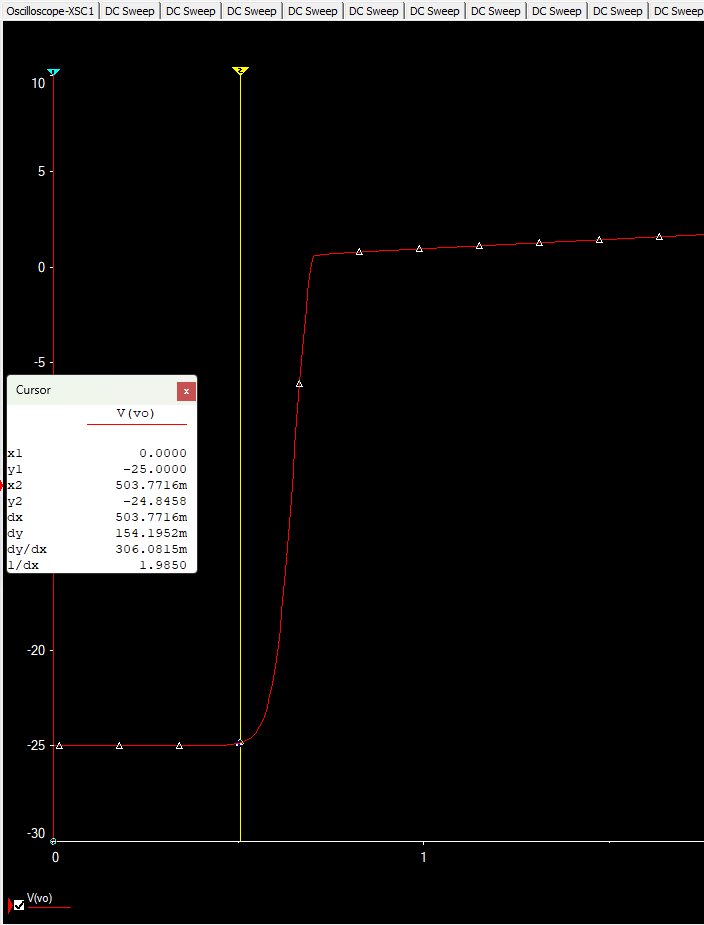
\includegraphics[width=\linewidth]{./my-chapters/my-images/Question2/a_VBE.png}
\end{minipage}
\begin{minipage}{.4\linewidth}
	\begin{itemize}[label=-]
		\item $v_{EB}<V_{EB(ON)}$: BJT hoạt động ở trạng thái \textbf{cut-off}
		\item $v_{EB}=V_{EB(ON)}=0.5038\,\textsf{V}$: BJT hoạt động ở trạng thái \textbf{active}
	\end{itemize}
\end{minipage}

\begin{minipage}{.4\linewidth}
	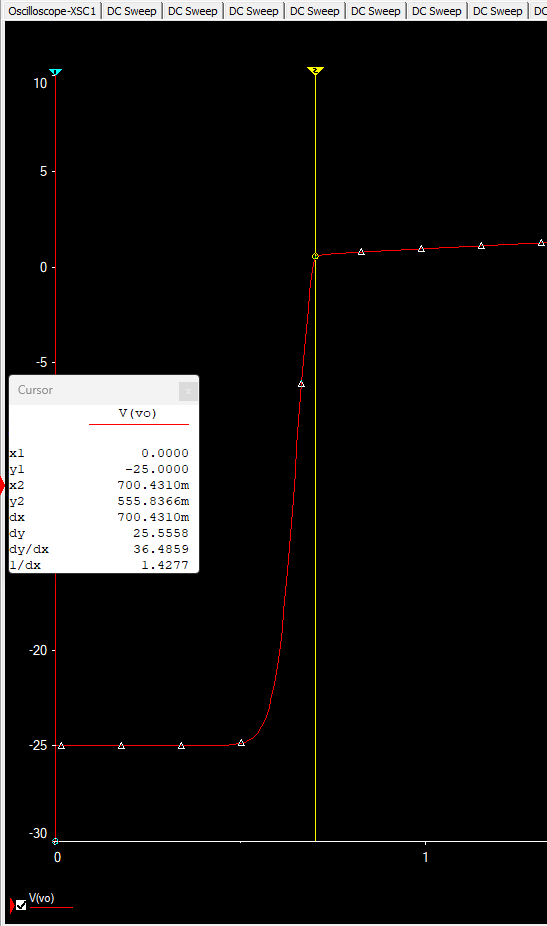
\includegraphics[width=\linewidth]{./my-chapters/my-images/Question2/a_VBE_sat.png}
\end{minipage}
\begin{minipage}{.4\linewidth}
	\begin{itemize}[label=-]
		\item $v_{EB}\geq\left.V_{EB}\right|_{v_{EC}={v_{EC}}_{sat}} = 0.7004\,\textsf{V}$: BJT hoạt động ở trạng thái \textbf{saturation}
	\end{itemize}
\end{minipage}

Tìm \textbf{điểm hoạt động Q}:
Áp dụng KVL cho vòng 1:
\[
- V_{EE}+R_{E}I_{E}+V_{EB}=0
\]
\[
\Rightarrow I_{E}=\frac{V_{EE}-V_{EB}}{R_{E}}=\frac{20-0.5038}{10\,\textsf{k}}=1.95\,\textsf{mA}
\]
\[
\Rightarrow I_{C}=\frac{\beta}{\beta+1}\times I_{E}=1.93\,\textsf{mA}
\]

Áp dụng KVL cho vòng 2:
\[
- V_{EE}+I_{E}(R_{E}+R_{C})+V_{EC}-V_{CC}=0
\]
\[
\Rightarrow V_{EC}=12.8392\,\textsf{V}
\]

Vậy điểm làm việc $Q$ là: \finalresult{\left(I_{CQ},V_{ECQ}\right)=\left(1.93\,\textsf{mA},\,12.8392\,\textsf{V}\right)}.

Kiểm tra kết quả
\begin{figure}[H]
	\centering
	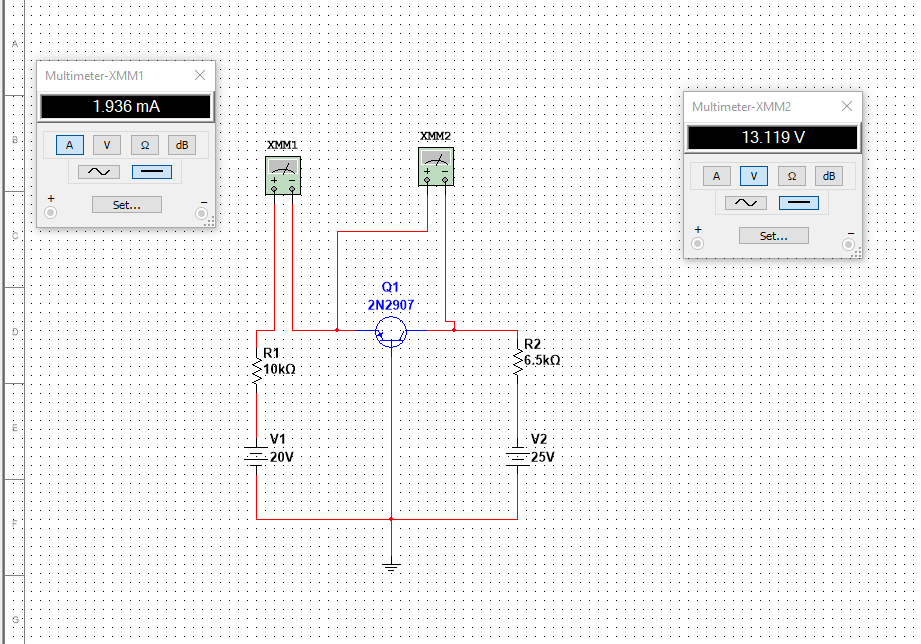
\includegraphics[width=\linewidth]{./my-chapters/my-images/Question2/Câu 2 a.png}
	\caption{Điểm phân cực $Q$ của mạch.}
\end{figure}

\answer{b}{Đặt $v_{1} = V_{m} \sin \left( \omega t\right)$ vào mạch. Tìm $A_{vo}$, $G_v$, $R_i$, $R_o$ của mạch.}

\[
g_{m}=\frac{I_{C}}{V_{T}}=77.2\,\textsf{mS}
\]
\[
R_{i}=\frac{1}{g_{m}}//R_{E}=\frac{\frac{1}{77.2\,\textsf{m}}\times10\,\textsf{k}}{\frac{1}{77.2\,\textsf{m}}+10\,\textsf{k}}=12.9366\,\Omega
\]
$\Rightarrow$ \finalresult{R_{i}=12.9366\,\Omega}.

\[
R_{o}=R_{C}=6.5\,\textsf{k}\Omega
\]
$\Rightarrow$ \finalresult{R_{o}=6.5\,\textsf{k}\Omega}.

\[
A_{vo}=g_{m}R_{C}=501.8\,\textsf{V/V}
\]
$\Rightarrow$ \finalresult{A_{vo}=501.8\,\textsf{V/V}}.

\[
A_{v}=A_{vo}\times\frac{R_{L}}{R_{o}+R_{L}}=501.8\times\frac{5\,\textsf{k}}{5\,\textsf{k}+6.5\,\textsf{k}}=218.1374\,\textsf{V/V}
\]
$\Rightarrow$ \finalresult{A_{v}=218.1374\,\textsf{V/V}}.

\[
G_{v}=A_{vo}\times\frac{R_{L}}{R_{o}+R_{L}}\times\frac{R_{i}}{R_{sig}+R_{i}}=501.8\times\frac{5\,\textsf{k}}{5\,\textsf{k}+6.5\,\textsf{k}}\times\frac{12.9366}{1\,\textsf{k}+12.9366}=2.79\,\textsf{V/V}
\]
$\Rightarrow$ \finalresult{G_{v}=2.79\,\textsf{V/V}}.

\begin{figure}[H]
	\centering
	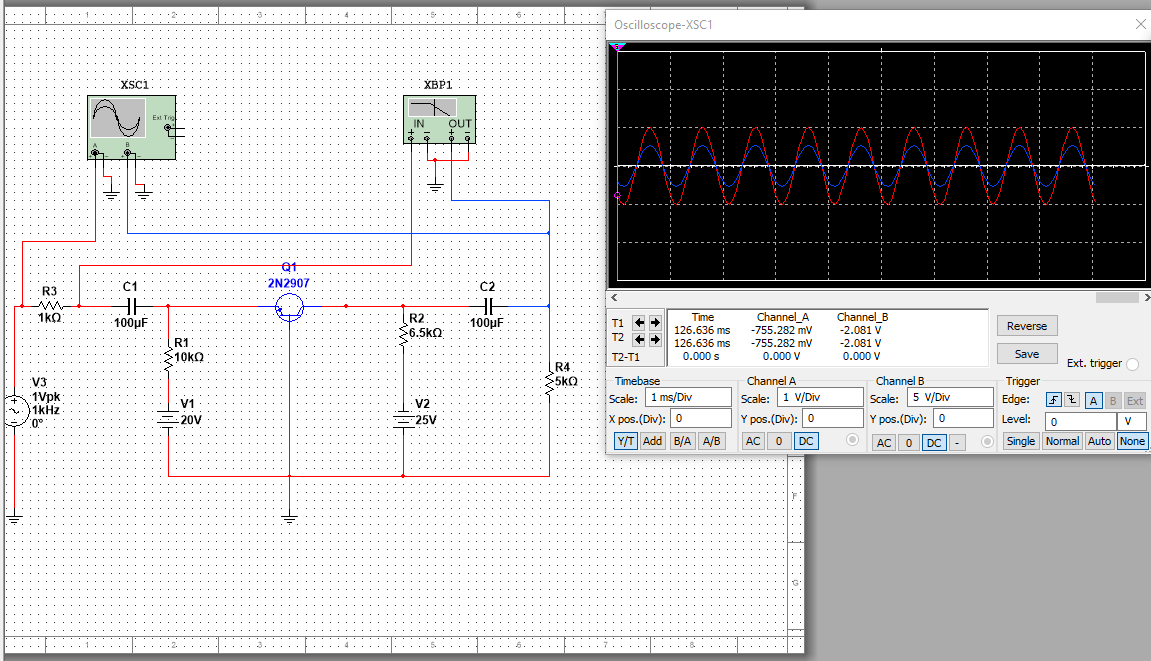
\includegraphics[width=\linewidth]{./my-chapters/my-images/Question2/Câu 2 b - Sóng .png}
	\caption{Dạng sóng ngõ vào và ngõ ra của mạch.}
\end{figure}

\begin{figure}[H]
	\centering
	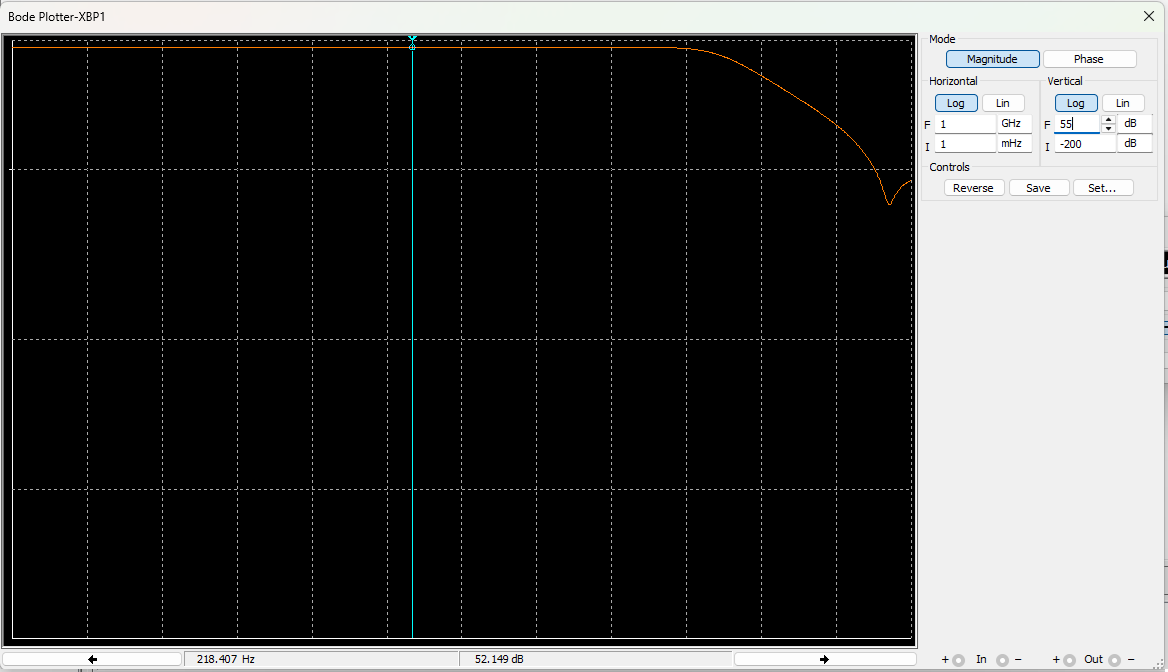
\includegraphics[width=\linewidth]{./my-chapters/my-images/Question2/b_avo.png}
	\caption{Đo $A_{vo} = 52.149\, dB \approx 404.9953$.}
\end{figure}

\begin{figure}[H]
	\centering
	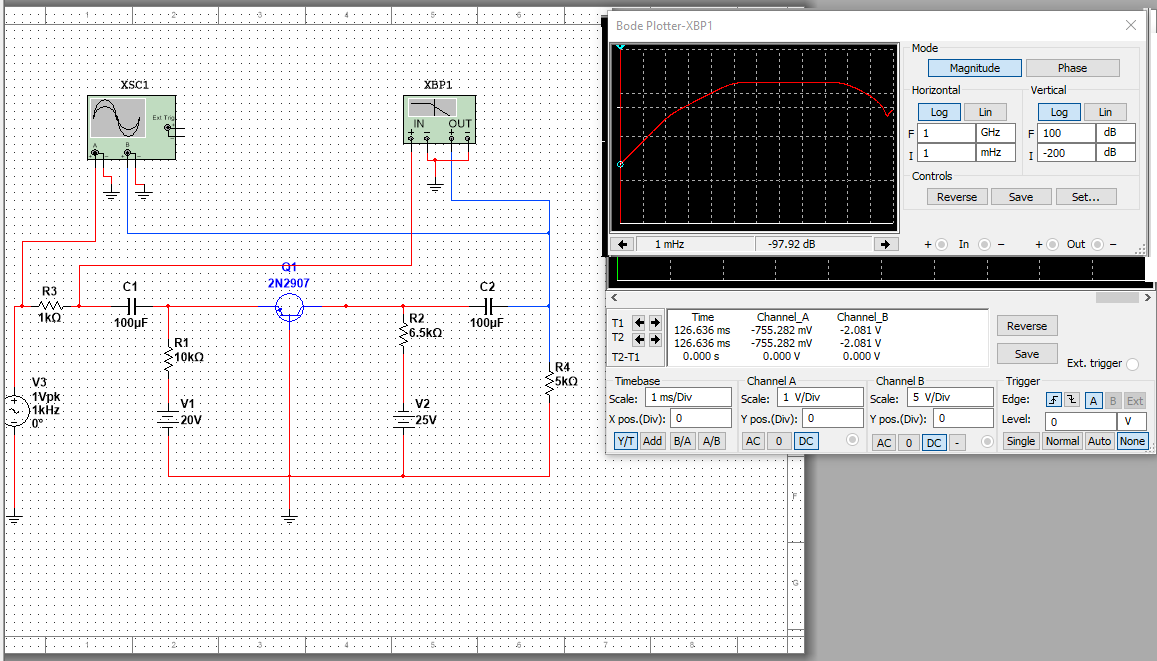
\includegraphics[width=\linewidth]{./my-chapters/my-images/Question2/Câu 2 b - Sóng và Av.png}
	\caption{Đo $A_{v} = 45.348dB \approx 185.0973$.}
\end{figure}

\begin{figure}[H]
	\centering
	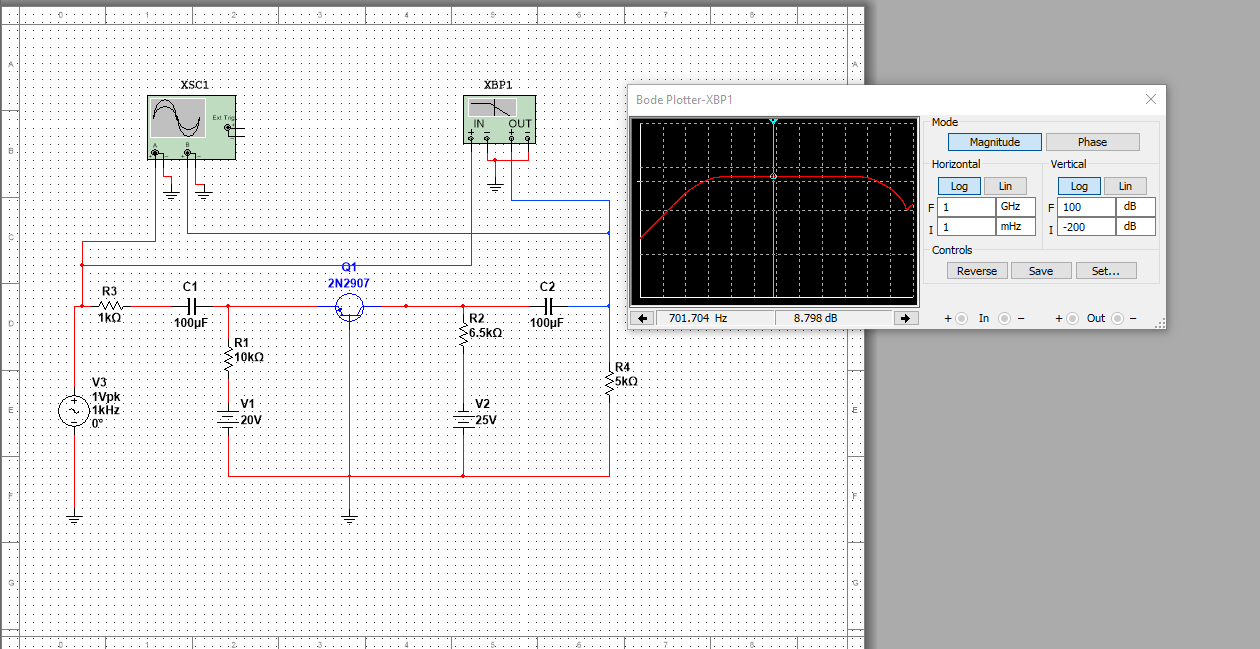
\includegraphics[width=\linewidth]{./my-chapters/my-images/Question2/Câu 2 b - Gv.png}
	\caption{Đo $G_{v} = 8.798\, dB \approx 2.7536$.}
\end{figure}

\answer{c}{Lựa chọn các tụ $C_{1}$, $C_{2}$ để mạch có $f_{L}=100\,\textsf{Hz}$.}

\begin{itemize}[label=-]
	\item Xét ảnh hưởng tụ $C_{1}$: 
	\[
	R_{C_{1}} = R_{sig} // R_{in}
	\Longrightarrow 
	\omega_{p_{1}} = \frac{1}{C_{1}\left(R_{sig} // R_{in} \right)}
	\]
	\item Xét ảnh hưởng tụ $C_{2}$: 
	\[
	R_{C_{2}} = R_{C} + R_{L}
	\Longrightarrow 
	\omega_{p_{2}} = \frac{1}{C_{2}\left(R_{C} + R_{L}\right)}
	\]
\end{itemize}

Theo phương pháp \textbf{cực tần số trội (dominant pole)}, chọn $C_{1}$ làm cực trội có giá trị $100\,\textsf{Hz}$, 
$C_{2}$ tạo ra cực ở tần số $40\,\textsf{Hz}$.  
Như vậy, tần số cắt của mạch là:
\[
f_{L} = \sqrt{f_{C_{1}}^{2} + f_{C_{2}}^{2}}
\]

\textbf{Lựa chọn các tụ $C_{1}$ và $C_{2}$:}
\[
C_{1} = \frac{1}{2\pi \times 100 \times (1\,\textsf{k}//12.9366)}
= 124.618\,\mu\textsf{F}
\]
\[
C_{2} = \frac{1}{2\pi \times 40 \times (6.5\,\textsf{k} + 5\,\textsf{k})}
= 0.36\,\mu\textsf{F}
\]

$\Rightarrow$ \finalresult{C_{1} = 124.618\,\mu\textsf{F}} và \finalresult{C_{2} = 0.36\,\mu\textsf{F}}.

Kiểm tra kết quả

\begin{figure}[H]
	\centering
	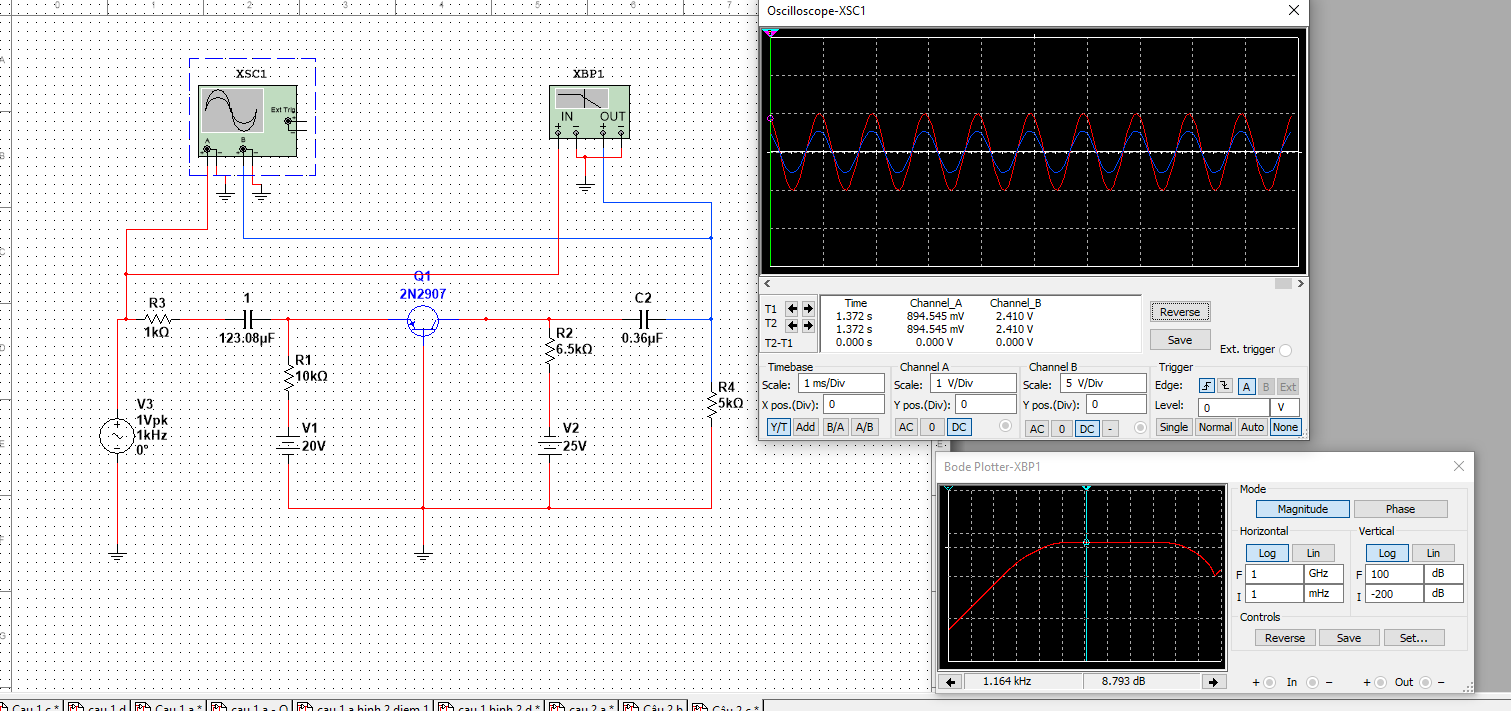
\includegraphics[width=\linewidth]{./my-chapters/my-images/Question2/Câu 2 d.png}
\end{figure}
